\documentclass[a4paper, 11pt]{scrreprt}
\usepackage[utf8]{inputenc}
\usepackage[ngerman]{babel}
\usepackage[T1]{fontenc}
\usepackage{lmodern}
\usepackage{amsmath,amssymb,amstext,amsfonts,mathrsfs}
\usepackage{graphicx}
\usepackage{color}

\usepackage{marginnote}

\pagestyle{headings}

\newtheorem{defi}{Definition}[section]
\newtheorem{prop}[defi]{Proposition}
\newtheorem{satz}[defi]{Satz}
\newtheorem{koro}[defi]{Korollar}
\newtheorem{lemma}[defi]{Lemma}

\newenvironment{beweis}[1][Beweis]{\begin{trivlist}
	\item[\hskip \labelsep {\bfseries #1}]}
	{\end{trivlist}}

\newcommand{\RR}{\mathbb{R}}
\newcommand{\EE}{\mathbb{E}}
\newcommand{\NN}{\mathbb{N}}

\newcommand{\student}[1]{\marginnote{{\normalfont\bf #1}}}

\title{Fallstudien der math. Modellbildung}
\author{Manuela Lambacher, Dominik Otto, Andreas Wiedemann}
\date{\today}

\begin{document}
\parindent 0pt
\maketitle
\tableofcontents

\chapter{Wittaker-Shannon-Sampling Theorem}

\section{The Wittaker-Shannon-Sampling Theorem}
\section{Proof of the Theorem}
\section{Meaning, real-life applications and limitations}

\chapter{Das Marchenko-Pastur-Gesetz}

\section{Das Marchenko-Pastur-Gesetz}

Sei \(Y_N\) eine \(N\times M(N)\)-Matrix mit unabhängigen zentrierten Einträgen mit Varianz \(1\),
	\[\sup_{j,k,N} \EE\left[ | Y_N(j,k)|^q\right] = C_q < \infty \qquad \forall q \in \NN\]
und \(M(N) \in \NN\) so, dass
	\[\lim_{N\to\infty} \frac{M(N)}{N} = \alpha \in[1,\infty). \]
Sei weiterhin die Wishart-Matrix gegeben als 
	\[W_N = \frac{1}{N}Y_NY_N^T,\]
und habe die empirische Eigenwertverteilung
	\[L_N = \frac{1}{n} \sum_{j=1}^{N} \delta_{\lambda_j} \]
und das Zustandsdichtemaß \(\overline{L_N} = \EE[L_N]\). Dann gilt die Konvergenz
	\[\overline{L_N} \xrightarrow{\text{w}} f_{\alpha}(x)dx \quad(N\to\infty)\]
im Raum der Wahrscheinlichkeitsmaße auf \(\RR\), wobei
	\[f_{\alpha}(x)=\frac{1}{2\pi x}\sqrt{(x-(1-\sqrt{\alpha})^2_{+}((1+\sqrt{\alpha})^2_{+}} \]

\newpage
\begin{beweis}
\begin{align*}
		N^{l+1} &\langle \overline{L_N}, x^l \rangle\ 
		= N^{l+1} \cdot \int x^l \overline{L_N}(dx) 
		= N^{l+1} \cdot \frac{1}{N} \cdot \EE[tr(W^l_N)] 
		= N^l \sum_{j_1,...,j_l = 1}^N \EE\left[\prod_{p = 1}^l W_{j_p,j_{p+1}}\right] \\
		&= N^l \sum_{j_1,...,j_l = 1}^N \EE\left[\prod_{p = 1}^l \frac{1}{N} \sum_{k = 1}^{M(N)} Y_N(j_p,k) \cdot Y_N(j_{p+1},k) \right] \\
		&= \sum_{j_1,...,j_l = 1}^N \EE \left[\left(\sum_{k = 1}^{M(N)} Y_N(j_1,k) \cdot Y_N(j_2,k)\right) \cdot \left(\prod_{p = 2}^l \sum_{k = 1}^{M(N)} Y_N(j_p,k) \cdot Y_N(j_{p+1},k) \right) \right] \\
		&= \sum_{j_1,...,j_l = 1}^N \EE\left[	\prod_{p = 2}^l \sum_{k_1,k_2 = 1}^{M(N)} Y_N(j_1,k_1) \cdot Y_N(j_2,k_1) \cdot Y_N(j_p,k_2) \cdot Y_N(j_{p+1},k_2) \right] \\
		&= ... \\
		&= \sum_{j_1,...,j_l = 1}^N \sum_{k_1,...,k_l = 1}^{M(N)} \EE[Y_N(j_1,k_1) Y_N(j_2,k_1) Y_N(j_2,k_2) Y_N(j_3,k_2) ... Y_N(j_l,k_l) Y_N(j_1,k_l)]
\end{align*}

Meine Ideen, wie es weiter geht. Hakt noch ein bisschen, sollte aber in die richtige Richtung gehen :)

\begin{equation}
 = \sum_{r_1,r_2 = 1}^l \sum_{\substack{J:v(J)=r_1\\ K:v(K)=r_2 }} \EE[Y_N(J,K)]
\end{equation}
Die einzelnen Summanden können also als Eulergraphen auf \(r_1+r_2 \)Knoten und \(2l\) Kanten interpretiert werden.
Damit ergeben sich die drei Fälle (setze \(r = r_1+r_2\) )
\begin{itemize}
	\item \(r < l+ 1\)\\
		\begin{align*}
			\EE[Y_N(J,k)] &\leq \prod_{n=1}^l \left(\sup_{j,k,N}\EE\left[|Y_N(j,k)|^l\right]\right)^{\frac 1 l} \\
			& = \prod_{n=1}^l C_l^{\frac 1 l} = C_l
			\end{align*}
	Außerdem: 
		\begin{align*}
			\#\{J: v(J)=r_1\} &\leq \begin{pmatrix} N \\ r_1 \end{pmatrix} r_1^l \leq N^{r_1}r_1^l \\
			\#\{K: v(K)=r_2\} &\leq \begin{pmatrix} M(N) \\ r_2 \end{pmatrix} r_2^l \leq M(N)^{r_2}r_2^l
		\end{align*}
	Somit gilt: 
		\[\frac {1}{N^{l+1}} \sum_{\substack{J:v(J)=r_1\\ K:v(K)=r_2 }} \EE[Y_N(J,K)] < C_l (l+1)^l \frac{N^{r_1} M(N)^{r_2}}{N^{l+1}} \xrightarrow{N\to\infty} 0\]
		
	\item \(r> l+1\) \\
		Nach Lemma aus der Vorlesung exisitert eine einfache, echte Kante und somit \(\EE[Y_N(J,K)]=0\)
	\item \(r=l+1\)\\
		Es tragen also nur die Graphen auf \(l+1\) verschiedenen Knoten zu \(\lim_{N\to\infty} \langle \overline{L_N}, x^l \rangle \) bei. Diese Graphen haben die Struktur eines Doppelbaumes, denen man geordnete, nicht überkreuzende Paarzerlegungen und damit auch Catalanpfade zuordnen kann.
\end{itemize}
\textbf{Weitere Analyse von \(\beta_l\):}\\
Wähle für einen Doppelbaum \(r\) Knoten aus den \(k\)-Knoten und \(l+1-r\) Knoten aus den \(j\)-Knoten. Dann folgt:
\begin{align*}
	\sum_{J,K: v(J)+v(K) = l+1} \EE[Y_N(J,K)] = &\sum_{r=1}^{l}\begin{pmatrix} N\\ l+1-r\end{pmatrix} (l+1-r)! \begin{pmatrix} M(N)\\r\end{pmatrix} r! \\
	&\cdot \#\{\text{Doppelbäume mit }l+1-r\ j\text{-Knoten und } r\ k\text{-Knoten}\} \\
	=& \sum_{r=1}^{l} \begin{pmatrix} N\\ l+1-r\end{pmatrix} (l+1-r)! \begin{pmatrix} M(N)\\r\end{pmatrix} r! \cdot C_l
\end{align*}
Ein Doppelbaum mit \((r)\  k\)-Knoten und \((l+1-r)\ j\)-Knoten kann wie folgt als Catalan-Pfad der Länge \(l\) interpretiert werden:\\
Wähle als Wurzel des Baumes einen \(j\)-Knoten und gliedere den Baum in Ebenen, wobei die Wurzel in der 0.Ebene liegt.(Die k-Knoten liegen also in ungeraden Ebenen, die j-Knoten in geradenen Ebenen) Verweise jede Kante mit einer Richtung, sodass bei jeder Doppelkante eine Kante von dem Knoten wegführt und eine zu ihm hinführt. Konstruiere den Catalan-Pfad wie folgt:\\
\begin{itemize}
	\item Alle Kanten zwischen der Wurzel und der ersten Ebene sind Flachstücke (+0)
	\item Wenn eine Kante von ungerader Ebene aufwärts auf gerade Ebene führt: \(+1\)
	\item Wenn eine Kante von gerader Ebene abwärts auf ungerade Ebene führt: \(-1\)
	\item Die restlichen Kanten sind alle Flachstücke
\end{itemize}
Beispiel: \\
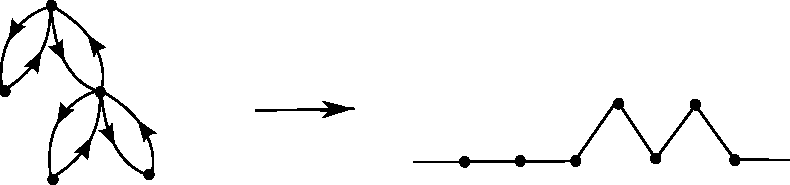
\includegraphics{Catalan-Pfad}
Lässt man die Wurzel außen vor, liegen \(r\ k\)-Knoten in den ungeraden Ebenen und \(l-r\ j\)-Knoten in den geraden Ebenen. Damit ergibt sich aus dieser Konstruktion, dass \(l-r\) die Anzahl der Aufstiege (und Abstiege) und \(2r\) die Anzahl der Flachstücke im Catalan-Pfad sind.  Denn: zu jedem \(j\)-Knoten führt genau eine Kante aus einer unteren Ebene hin und es führt genau eine Kante in eine untere Ebene zurück (Doppelbaum!). \\
\\ Die Abbildung von den Doppelbäumen auf die Catalanpfade ist eine Bijektion, da:
\begin{itemize}
 \item[•]Da der Graph eulersch ist, ist $ \sum_{i=1}^{2l} $ =0; Der Graph ist immer über 0, ansonsten würde es ein m geben, sodass $ \sum_{i=1}^{2m-1}s^{i}=-1, ~\sum_{i=1}^{2m}s^{i}=0, ~ s_{2m-1}=-1  $. Also könnten wir einen Doppelbaum mit Knoten {1,2,...2m} konstruieren, und da $ s_{2m-1}=-1  $ ist, würde eine Kante von diesem Knoten zurück zu einem der ersten 2m Knoten gehen, was dem Aufbau eines Doppelbaums widersprechen würde. Insgesamt haben wir also einen Catalanpfad konstruiert. 
 \item[•] Surjektivität:  für jeden Catalanpfad der Länge l der Form $\lbrace s_{i} \rbrace$, $ i \leq 2l, i \in \NN $ kann ein Doppelbaum als Urbild wie folgt konstruiert werden: für i gerade: $s_{i}=-1 \rightarrow $ gehe von $j_{i/2}$abwärts, bei $s_{i}=0  $ aufwärts; für i ungerade bei $s_{i}=1 $ aufwärts, bei $s_{i}=0 $ abwärts. 
\item[•] Injektivität analog zur Übung (bzw muss man das unbedingt nochmal zeigen?)\\
\end{itemize}
Die betrachteten Doppelbäume haben s.o. ein kombinatorisches Gewicht von 
	\[ \begin{pmatrix} N\\ l+1-r\end{pmatrix} (l+1-r)! \begin{pmatrix} M(N)\\r\end{pmatrix} r! \]
Für N hinreichend groß ist dies genähert \(N^{l+1-r}M(N)^r\). Damit folgt:
	\[\frac {1}{N^{l+1}} N^{l+1-r}M(N)^r =~ \left( \dfrac{M(N)}{N}\right)^{r}\to \alpha^r\]
und damit:
	\begin{align*}
		\beta_l &= \lim_{N \to \infty} \sum_{J,K: v(J)+v(K) = l+1} \dfrac{1}{N^{l+1}}\EE[Y_N(J,K)] = \sum_{r=1}^{l} \alpha^r\ C_{l} \\
		&= \sum_{p\in C_l} \alpha^r
	\end{align*}
wobei \(r = \frac 1 2 \#\{\text{Flachstücke in }C_l\} = l  - \#\{\text{Anstiege in }  C_l\}\).

Gleichung (10) würde ich versuchen per Induktion zu beweisen (Es geht sicher schöner, aber ich weiß nicht wie /ebenfalls nicht, es schreit aber auch nach Induktion;), ich hänge aber noch beim Induktionsschritt.  \\
$ \gamma_{l} $ sind die Aufstiege/Abstiege im Doppelbaum.\\
Induktionsanfang: \(l=1\): 
	\[\beta_1 = \alpha\gamma_1=\alpha\beta_0 \gamma_0=\alpha\]
	
Induktionsschritt: Ich denke, dass aus der Rekursionsformel für Catalanzahlen \(C_{l+1} = \sum_{k=0}^l C_kC_{l-k}\) folgt, dass
	\[\beta_{l+1} = \sum_{k=0}^l \beta_k\beta_{l-k} = \alpha \sum_{k=0}^l \beta_k\gamma_{l-k}\]
aber das ist eher wage...
Wir brauchen wh sogar zweimal Induktion einmal für $ \beta = \alpha \gamma $ und einmal für $ \gamma= \sum \beta \gamma $..\\

\textbf{Formel (12)}\\
\begin{align}
	Q_n =& \alpha^{-1-n/2}\int_{\RR} f_{\alpha}(x)x(x-\alpha -1)^n\,\mathrm{d}x \\
	 =& \frac{1}{2\pi}\alpha^{-1-n/2} \int_{(1-\sqrt{\alpha})^2}^{(1+\sqrt{\alpha})^2} \sqrt{(x-(1-\sqrt{\alpha})^2)((1+\sqrt{\alpha})^2-x)} (x-\alpha -1)^n \,\mathrm{d}x\\
	=& \frac{1}{2\pi}\alpha^{-1-n/2} \int_{(1-\sqrt{\alpha})^2}^{(1+\sqrt{\alpha})^2} \sqrt{-\alpha^2+2\alpha x+2\alpha -x^2+2x-1}(x-\alpha-1)^n \,\mathrm{d}x\\
	\overset{x=y+\alpha+1}{=}& \frac{1}{2\pi}\alpha^{-1-n/2} \int_{-2\sqrt{\alpha}}^{2\sqrt{\alpha}} \sqrt{4\alpha -y^2} y^n \,\mathrm{d}y\\
	\overset{y=2\sqrt{\alpha}z}{=}& \frac{1}{2\pi}\alpha^{-1-n/2} \cdot 2^n \alpha^{n/2}\cdot4\sqrt{\alpha}\int_{-1}^{1} \sqrt{1-z^2}z^n \,\mathrm{d}z = \frac{2}{\pi} \cdot 2^n\int_{-1}^{1} \sqrt{1-z^2}z^n\,\mathrm{d}z \\
	\overset{\text{Übung 1}}{=}& \sigma(z^n) = \begin{cases} 0, &n\text{ ungerade}\\
	C_{\frac l 2}, &n\text{gerade} \end{cases}
\end{align}
(Falls wir noch Platz füllen müssen, können wir hier die Rechnung aus der Übung auch wiederholen ;) )
Bei den "`Verständnis-Fragen"' habe ich jedoch etwas Probleme: \(f_{\alpha}\) ist für x=0 gar nicht definiert? Durch die Rechnung ergibt sich aber der Bezug zu \(\sigma(x)\), wo man dann doch beim Halbkreisgesetz wäre.\\
Zur Eindeutigkeit von \(f_{\alpha}\) sind diese "`verallgemeinerten Momente"' ein Problem. Habt ihr in der großen W-Theorie Vorlesung dazu was gemacht?



\end{beweis}


\end{document}
